\chapter{Italy: Sinbad the Sailor}

Towards the beginning of the year 1838, two young men belonging to the
first society of Paris, the Viscount Albert de Morcerf and the Baron
Franz d’Épinay, were at Florence. They had agreed to see the Carnival
at Rome that year, and that Franz, who for the last three or four years
had inhabited Italy, should act as \textit{cicerone} to Albert.

As it is no inconsiderable affair to spend the Carnival at Rome,
especially when you have no great desire to sleep on the Piazza del
Popolo, or the Campo Vaccino, they wrote to Signor Pastrini, the
proprietor of the Hôtel de Londres, Piazza di Spagna, to reserve
comfortable apartments for them. Signor Pastrini replied that he had
only two rooms and a parlor on the third floor, which he offered at the
low charge of a louis per diem. They accepted his offer; but wishing to
make the best use of the time that was left, Albert started for Naples.
As for Franz, he remained at Florence, and after having passed a few
days in exploring the paradise of the Cascine, and spending two or
three evenings at the houses of the Florentine nobility, he took a
fancy into his head (having already visited Corsica, the cradle of
Bonaparte) to visit Elba, the waiting-place of Napoleon.

One evening he cast off the painter of a sailboat from the iron ring
that secured it to the dock at Leghorn, wrapped himself in his coat and
lay down, and said to the crew,—“To the Island of Elba!”

The boat shot out of the harbor like a bird and the next morning Franz
disembarked at Porto-Ferrajo. He traversed the island, after having
followed the traces which the footsteps of the giant have left, and
re-embarked for Marciana.

Two hours after he again landed at Pianosa, where he was assured that
red partridges abounded. The sport was bad; Franz only succeeded in
killing a few partridges, and, like every unsuccessful sportsman, he
returned to the boat very much out of temper.

“Ah, if your excellency chose,” said the captain, “you might have
capital sport.”

“Where?”

“Do you see that island?” continued the captain, pointing to a conical
pile rising from the indigo sea.

“Well, what is this island?”

“The Island of Monte Cristo.”

“But I have no permission to shoot over this island.”

“Your excellency does not require a permit, for the island is
uninhabited.”

“Ah, indeed!” said the young man. “A desert island in the midst of the
Mediterranean must be a curiosity.”

“It is very natural; this island is a mass of rocks, and does not
contain an acre of land capable of cultivation.”

“To whom does this island belong?”

“To Tuscany.”

“What game shall I find there!”

“Thousands of wild goats.”

“Who live upon the stones, I suppose,” said Franz with an incredulous
smile.

“No, but by browsing the shrubs and trees that grow out of the crevices
of the rocks.”

“Where can I sleep?”

“On shore in the grottos, or on board in your cloak; besides, if your
excellency pleases, we can leave as soon as you like—we can sail as
well by night as by day, and if the wind drops we can use our oars.”

As Franz had sufficient time, and his apartments at Rome were not yet
available, he accepted the proposition. Upon his answer in the
affirmative, the sailors exchanged a few words together in a low tone.
“Well,” asked he, “what now? Is there any difficulty in the way?”

“No.” replied the captain, “but we must warn your excellency that the
island is an infected port.”

“What do you mean?”

“Monte Cristo although uninhabited, yet serves occasionally as a refuge
for the smugglers and pirates who come from Corsica, Sardinia, and
Africa, and if it becomes known that we have been there, we shall have
to perform quarantine for six days on our return to Leghorn.”

“The deuce! That puts a different face on the matter. Six days! Why,
that’s as long as the Almighty took to make the world! Too long a
wait—too long.”

“But who will say your excellency has been to Monte Cristo?”

“Oh, I shall not,” cried Franz.

“Nor I, nor I,” chorused the sailors.

“Then steer for Monte Cristo.”

The captain gave his orders, the helm was put up, and the boat was soon
sailing in the direction of the island. Franz waited until all was in
order, and when the sail was filled, and the four sailors had taken
their places—three forward, and one at the helm—he resumed the
conversation. “Gaetano,” said he to the captain, “you tell me Monte
Cristo serves as a refuge for pirates, who are, it seems to me, a very
different kind of game from the goats.”

“Yes, your excellency, and it is true.”

“I knew there were smugglers, but I thought that since the capture of
Algiers, and the destruction of the regency, pirates existed only in
the romances of Cooper and Captain Marryat.”

“Your excellency is mistaken; there are pirates, like the bandits who
were believed to have been exterminated by Pope Leo XII., and who yet,
every day, rob travellers at the gates of Rome. Has not your excellency
heard that the French \textit{chargé d’affaires} was robbed six months ago
within five hundred paces of Velletri?”

“Oh, yes, I heard that.”

“Well, then, if, like us, your excellency lived at Leghorn, you would
hear, from time to time, that a little merchant vessel, or an English
yacht that was expected at Bastia, at Porto-Ferrajo, or at Civita
Vecchia, has not arrived; no one knows what has become of it, but,
doubtless, it has struck on a rock and foundered. Now this rock it has
met has been a long and narrow boat, manned by six or eight men, who
have surprised and plundered it, some dark and stormy night, near some
desert and gloomy island, as bandits plunder a carriage in the recesses
of a forest.”

“But,” asked Franz, who lay wrapped in his cloak at the bottom of the
boat, “why do not those who have been plundered complain to the French,
Sardinian, or Tuscan governments?”

“Why?” said Gaetano with a smile.

“Yes, why?”

“Because, in the first place, they transfer from the vessel to their
own boat whatever they think worth taking, then they bind the crew hand
and foot, they attach to everyone’s neck a four-and-twenty-pound ball,
a large hole is chopped in the vessel’s bottom, and then they leave
her. At the end of ten minutes the vessel begins to roll heavily and
settle down. First one gun’l goes under, then the other. Then they lift
and sink again, and both go under at once. All at once there’s a noise
like a cannon—that’s the air blowing up the deck. Soon the water rushes
out of the scupper-holes like a whale spouting, the vessel gives a last
groan, spins round and round, and disappears, forming a vast whirlpool
in the ocean, and then all is over, so that in five minutes nothing but
the eye of God can see the vessel where she lies at the bottom of the
sea. Do you understand now,” said the captain, “why no complaints are
made to the government, and why the vessel never reaches port?”

It is probable that if Gaetano had related this previous to proposing
the expedition, Franz would have hesitated, but now that they had
started, he thought it would be cowardly to draw back. He was one of
those men who do not rashly court danger, but if danger presents
itself, combat it with the most unalterable coolness. Calm and
resolute, he treated any peril as he would an adversary in a
duel,—calculated its probable method of approach; retreated, if at all,
as a point of strategy and not from cowardice; was quick to see an
opening for attack, and won victory at a single thrust.

“Bah!” said he, “I have travelled through Sicily and Calabria—I have
sailed two months in the Archipelago, and yet I never saw even the
shadow of a bandit or a pirate.”

“I did not tell your excellency this to deter you from your project,”
replied Gaetano, “but you questioned me, and I have answered; that’s
all.”

“Yes, and your conversation is most interesting; and as I wish to enjoy
it as long as possible, steer for Monte Cristo.”

The wind blew strongly, the boat made six or seven knots an hour, and
they were rapidly reaching the end of their voyage. As they drew near
the island seemed to lift from the sea, and the air was so clear that
they could already distinguish the rocks heaped on one another, like
cannon balls in an arsenal, with green bushes and trees growing in the
crevices. As for the sailors, although they appeared perfectly tranquil
yet it was evident that they were on the alert, and that they carefully
watched the glassy surface over which they were sailing, and on which a
few fishing-boats, with their white sails, were alone visible.

They were within fifteen miles of Monte Cristo when the sun began to
set behind Corsica, whose mountains appeared against the sky, showing
their rugged peaks in bold relief; this mass of rock, like the giant
Adamastor, rose dead ahead, a formidable barrier, and intercepting the
light that gilded its massive peaks so that the voyagers were in
shadow. Little by little the shadow rose higher and seemed to drive
before it the last rays of the expiring day; at last the reflection
rested on the summit of the mountain, where it paused an instant, like
the fiery crest of a volcano, then gloom gradually covered the summit
as it had covered the base, and the island now only appeared to be a
gray mountain that grew continually darker; half an hour after, the
night was quite dark.

Fortunately, the mariners were used to these latitudes, and knew every
rock in the Tuscan Archipelago; for in the midst of this obscurity
Franz was not without uneasiness—Corsica had long since disappeared,
and Monte Cristo itself was invisible; but the sailors seemed, like the
lynx, to see in the dark, and the pilot who steered did not evince the
slightest hesitation.

An hour had passed since the sun had set, when Franz fancied he saw, at
a quarter of a mile to the left, a dark mass, but he could not
precisely make out what it was, and fearing to excite the mirth of the
sailors by mistaking a floating cloud for land, he remained silent;
suddenly a great light appeared on the strand; land might resemble a
cloud, but the fire was not a meteor.

“What is this light?” asked he.

“Hush!” said the captain; “it is a fire.”

“But you told me the island was uninhabited?”

“I said there were no fixed habitations on it, but I said also that it
served sometimes as a harbor for smugglers.”

“And for pirates?”

“And for pirates,” returned Gaetano, repeating Franz’s words. “It is
for that reason I have given orders to pass the island, for, as you
see, the fire is behind us.”

“But this fire?” continued Franz. “It seems to me rather reassuring
than otherwise; men who did not wish to be seen would not light a
fire.”

“Oh, that goes for nothing,” said Gaetano. “If you can guess the
position of the island in the darkness, you will see that the fire
cannot be seen from the side or from Pianosa, but only from the sea.”

“You think, then, this fire indicates the presence of unpleasant
neighbors?”

“That is what we must find out,” returned Gaetano, fixing his eyes on
this terrestrial star.

“How can you find out?”

“You shall see.”

Gaetano consulted with his companions, and after five minutes’
discussion a manœuvre was executed which caused the vessel to tack
about, they returned the way they had come, and in a few minutes the
fire disappeared, hidden by an elevation of the land. The pilot again
changed the course of the boat, which rapidly approached the island,
and was soon within fifty paces of it. Gaetano lowered the sail, and
the boat came to rest. All this was done in silence, and from the
moment that their course was changed not a word was spoken.

Gaetano, who had proposed the expedition, had taken all the
responsibility on himself; the four sailors fixed their eyes on him,
while they got out their oars and held themselves in readiness to row
away, which, thanks to the darkness, would not be difficult. As for
Franz, he examined his arms with the utmost coolness; he had two
double-barrelled guns and a rifle; he loaded them, looked at the
priming, and waited quietly.

During this time the captain had thrown off his vest and shirt, and
secured his trousers round his waist; his feet were naked, so he had no
shoes and stockings to take off; after these preparations he placed his
finger on his lips, and lowering himself noiselessly into the sea, swam
towards the shore with such precaution that it was impossible to hear
the slightest sound; he could only be traced by the phosphorescent line
in his wake. This track soon disappeared; it was evident that he had
touched the shore.

Everyone on board remained motionless for half an hour, when the same
luminous track was again observed, and the swimmer was soon on board.

“Well?” exclaimed Franz and the sailors in unison.

“They are Spanish smugglers,” said he; “they have with them two
Corsican bandits.”

“And what are these Corsican bandits doing here with Spanish
smugglers?”

“Alas,” returned the captain with an accent of the most profound pity,
“we ought always to help one another. Very often the bandits are hard
pressed by gendarmes or carbineers; well, they see a vessel, and good
fellows like us on board, they come and demand hospitality of us; you
can’t refuse help to a poor hunted devil; we receive them, and for
greater security we stand out to sea. This costs us nothing, and saves
the life, or at least the liberty, of a fellow-creature, who on the
first occasion returns the service by pointing out some safe spot where
we can land our goods without interruption.”

“Ah!” said Franz, “then you are a smuggler occasionally, Gaetano?”

“Your excellency, we must live somehow,” returned the other, smiling
impenetrably.

“Then you know the men who are now on Monte Cristo?”

“Oh, yes, we sailors are like freemasons, and recognize each other by
signs.”

“And do you think we have nothing to fear if we land?”

“Nothing at all; smugglers are not thieves.”

“But these two Corsican bandits?” said Franz, calculating the chances
of peril.

“It is not their fault that they are bandits, but that of the
authorities.”

“How so?”

“Because they are pursued for having made a stiff, as if it was not in
a Corsican’s nature to revenge himself.”

“What do you mean by having made a stiff?—having assassinated a man?”
said Franz, continuing his investigation.

“I mean that they have killed an enemy, which is a very different
thing,” returned the captain.

“Well,” said the young man, “let us demand hospitality of these
smugglers and bandits. Do you think they will grant it?”

“Without doubt.”

“How many are they?”

“Four, and the two bandits make six.”

“Just our number, so that if they prove troublesome, we shall be able
to hold them in check; so, for the last time, steer to Monte Cristo.”

“Yes, but your excellency will permit us to take all due precautions.”

“By all means, be as wise as Nestor and as prudent as Ulysses; I do
more than permit, I exhort you.”

“Silence, then!” said Gaetano.

Everyone obeyed. For a man who, like Franz, viewed his position in its
true light, it was a grave one. He was alone in the darkness with
sailors whom he did not know, and who had no reason to be devoted to
him; who knew that he had several thousand francs in his belt, and who
had often examined his weapons,—which were very beautiful,—if not with
envy, at least with curiosity. On the other hand, he was about to land,
without any other escort than these men, on an island which had,
indeed, a very religious name, but which did not seem to Franz likely
to afford him much hospitality, thanks to the smugglers and bandits.
The history of the scuttled vessels, which had appeared improbable
during the day, seemed very probable at night; placed as he was between
two possible sources of danger, he kept his eye on the crew, and his
gun in his hand.

The sailors had again hoisted sail, and the vessel was once more
cleaving the waves. Through the darkness Franz, whose eyes were now
more accustomed to it, could see the looming shore along which the boat
was sailing, and then, as they rounded a rocky point, he saw the fire
more brilliant than ever, and about it five or six persons seated. The
blaze illumined the sea for a hundred paces around. Gaetano skirted the
light, carefully keeping the boat in the shadow; then, when they were
opposite the fire, he steered to the centre of the circle, singing a
fishing song, of which his companions sung the chorus.

At the first words of the song the men seated round the fire arose and
approached the landing-place, their eyes fixed on the boat, evidently
seeking to know who the new-comers were and what were their intentions.
They soon appeared satisfied and returned (with the exception of one,
who remained at the shore) to their fire, at which the carcass of a
goat was roasting. When the boat was within twenty paces of the shore,
the man on the beach, who carried a carbine, presented arms after the
manner of a sentinel, and cried, “Who comes there?” in Sardinian.

Franz coolly cocked both barrels. Gaetano then exchanged a few words
with this man which the traveller did not understand, but which
evidently concerned him.

“Will your excellency give your name, or remain \textit{incognito}?” asked the
captain.

“My name must rest unknown,” replied Franz; “merely say I am a
Frenchman travelling for pleasure.”

As soon as Gaetano had transmitted this answer, the sentinel gave an
order to one of the men seated round the fire, who rose and disappeared
among the rocks. Not a word was spoken, everyone seemed occupied, Franz
with his disembarkment, the sailors with their sails, the smugglers
with their goat; but in the midst of all this carelessness it was
evident that they mutually observed each other.

The man who had disappeared returned suddenly on the opposite side to
that by which he had left; he made a sign with his head to the
sentinel, who, turning to the boat, said, “\textit{S’accommodi}.” The Italian
\textit{s’accommodi} is untranslatable; it means at once, “Come, enter, you
are welcome; make yourself at home; you are the master.” It is like
that Turkish phrase of Molière’s that so astonished the bourgeois
gentleman by the number of things implied in its utterance.

The sailors did not wait for a second invitation; four strokes of the
oar brought them to land; Gaetano sprang to shore, exchanged a few
words with the sentinel, then his comrades disembarked, and lastly came
Franz. One of his guns was swung over his shoulder, Gaetano had the
other, and a sailor held his rifle; his dress, half artist, half dandy,
did not excite any suspicion, and, consequently, no disquietude. The
boat was moored to the shore, and they advanced a few paces to find a
comfortable bivouac; but, doubtless, the spot they chose did not suit
the smuggler who filled the post of sentinel, for he cried out:

“Not that way, if you please.”

Gaetano faltered an excuse, and advanced to the opposite side, while
two sailors kindled torches at the fire to light them on their way.

They advanced about thirty paces, and then stopped at a small esplanade
surrounded with rocks, in which seats had been cut, not unlike
sentry-boxes. Around in the crevices of the rocks grew a few dwarf oaks
and thick bushes of myrtles. Franz lowered a torch, and saw by the mass
of cinders that had accumulated that he was not the first to discover
this retreat, which was, doubtless, one of the halting-places of the
wandering visitors of Monte Cristo.

As for his suspicions, once on \textit{terra firma}, once that he had seen the
indifferent, if not friendly, appearance of his hosts, his anxiety had
quite disappeared, or rather, at sight of the goat, had turned to
appetite. He mentioned this to Gaetano, who replied that nothing could
be more easy than to prepare a supper when they had in their boat,
bread, wine, half a dozen partridges, and a good fire to roast them by.

“Besides,” added he, “if the smell of their roast meat tempts you, I
will go and offer them two of our birds for a slice.”

“You are a born diplomat,” returned Franz; “go and try.”

Meanwhile the sailors had collected dried sticks and branches with
which they made a fire. Franz waited impatiently, inhaling the aroma of
the roasted meat, when the captain returned with a mysterious air.

“Well,” said Franz, “anything new?—do they refuse?”

“On the contrary,” returned Gaetano, “the chief, who was told you were
a young Frenchman, invites you to sup with him.”

“Well,” observed Franz, “this chief is very polite, and I see no
objection—the more so as I bring my share of the supper.”

“Oh, it is not that; he has plenty, and to spare, for supper; but he
makes one condition, and rather a peculiar one, before he will receive
you at his house.”

“His house? Has he built one here, then?”

“No, but he has a very comfortable one all the same, so they say.”

“You know this chief, then?”

“I have heard talk of him.”

“Favorably or otherwise?”

“Both.”

“The deuce!—and what is this condition?”

“That you are blindfolded, and do not take off the bandage until he
himself bids you.”

Franz looked at Gaetano, to see, if possible, what he thought of this
proposal. “Ah,” replied he, guessing Franz’s thought, “I know this is a
serious matter.”

“What should you do in my place?”

“I, who have nothing to lose,—I should go.”

\begin{figure}[ht]
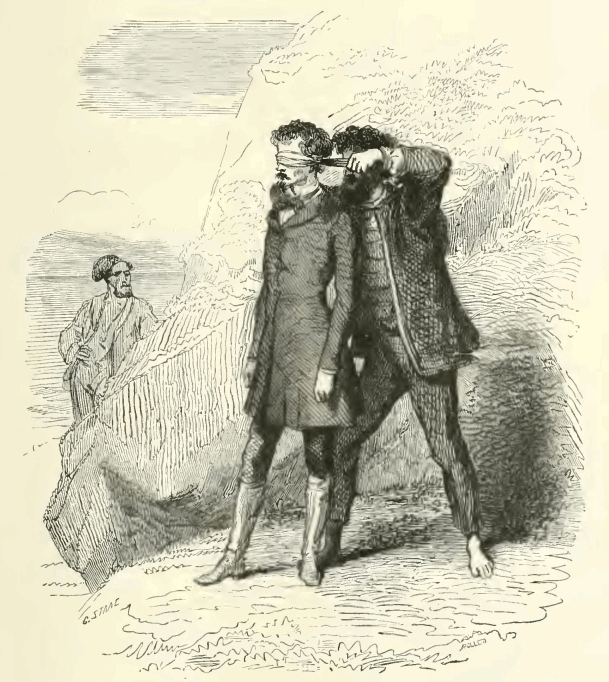
\includegraphics[width=\textwidth]{20075m.jpg}
\end{figure}

“You would accept?”

“Yes, were it only out of curiosity.”

“There is something very peculiar about this chief, then?”

“Listen,” said Gaetano, lowering his voice, “I do not know if what they
say is true”—he stopped to see if anyone was near.

“What do they say?”

“That this chief inhabits a cavern to which the Pitti Palace is
nothing.”

“What nonsense!” said Franz, reseating himself.

“It is no nonsense; it is quite true. Cama, the pilot of the \textit{Saint
Ferdinand}, went in once, and he came back amazed, vowing that such
treasures were only to be heard of in fairy tales.”

“Do you know,” observed Franz, “that with such stories you make me
think of Ali Baba’s enchanted cavern?”

“I tell you what I have been told.”

“Then you advise me to accept?”

“Oh, I don’t say that; your excellency will do as you please; I should
be sorry to advise you in the matter.”

Franz pondered the matter for a few moments, concluded that a man so
rich could not have any intention of plundering him of what little he
had, and seeing only the prospect of a good supper, accepted. Gaetano
departed with the reply. Franz was prudent, and wished to learn all he
possibly could concerning his host. He turned towards the sailor, who,
during this dialogue, had sat gravely plucking the partridges with the
air of a man proud of his office, and asked him how these men had
landed, as no vessel of any kind was visible.

“Never mind that,” returned the sailor, “I know their vessel.”

“Is it a very beautiful vessel?”

“I would not wish for a better to sail round the world.”

“Of what burden is she?”

“About a hundred tons; but she is built to stand any weather. She is
what the English call a yacht.”

“Where was she built?”

“I know not; but my own opinion is she is a Genoese.”

“And how did a leader of smugglers,” continued Franz, “venture to build
a vessel designed for such a purpose at Genoa?”

“I did not say that the owner was a smuggler,” replied the sailor.

“No; but Gaetano did, I thought.”

“Gaetano had only seen the vessel from a distance, he had not then
spoken to anyone.”

“And if this person be not a smuggler, who is he?”

“A wealthy signor, who travels for his pleasure.”

“Come,” thought Franz, “he is still more mysterious, since the two
accounts do not agree.”

“What is his name?”

“If you ask him, he says Sinbad the Sailor; but I doubt if it be his
real name.”

“Sinbad the Sailor?”

“Yes.”

“And where does he reside?”

“On the sea.”

“What country does he come from?”

“I do not know.”

“Have you ever seen him?”

“Sometimes.”

“What sort of a man is he?”

“Your excellency will judge for yourself.”

“Where will he receive me?”

“No doubt in the subterranean palace Gaetano told you of.”

“Have you never had the curiosity, when you have landed and found this
island deserted, to seek for this enchanted palace?”

“Oh, yes, more than once, but always in vain; we examined the grotto
all over, but we never could find the slightest trace of any opening;
they say that the door is not opened by a key, but a magic word.”

“Decidedly,” muttered Franz, “this is an Arabian Nights’ adventure.”

“His excellency waits for you,” said a voice, which he recognized as
that of the sentinel. He was accompanied by two of the yacht’s crew.

Franz drew his handkerchief from his pocket, and presented it to the
man who had spoken to him. Without uttering a word, they bandaged his
eyes with a care that showed their apprehensions of his committing some
indiscretion. Afterwards he was made to promise that he would not make
the least attempt to raise the bandage. He promised.

Then his two guides took his arms, and he went on, guided by them, and
preceded by the sentinel. After going about thirty paces, he smelt the
appetizing odor of the kid that was roasting, and knew thus that he was
passing the bivouac; they then led him on about fifty paces farther,
evidently advancing towards that part of the shore where they would not
allow Gaetano to go—a refusal he could now comprehend.

Presently, by a change in the atmosphere, he knew that they were
entering a cave; after going on for a few seconds more he heard a
crackling, and it seemed to him as though the atmosphere again changed,
and became balmy and perfumed. At length his feet touched on a thick
and soft carpet, and his guides let go their hold of him. There was a
moment’s silence, and then a voice, in excellent French, although, with
a foreign accent, said:

“Welcome, sir. I beg you will remove your bandage.”

It may be supposed, then, Franz did not wait for a repetition of this
permission, but took off the handkerchief, and found himself in the
presence of a man from thirty-eight to forty years of age, dressed in a
Tunisian costume, that is to say, a red cap with a long blue silk
tassel, a vest of black cloth embroidered with gold, pantaloons of deep
red, large and full gaiters of the same color, embroidered with gold
like the vest, and yellow slippers; he had a splendid cashmere round
his waist, and a small sharp and crooked cangiar was passed through his
girdle.

Although of a paleness that was almost livid, this man had a remarkably
handsome face; his eyes were penetrating and sparkling; his nose, quite
straight, and projecting direct from the brow, was of the pure Greek
type, while his teeth, as white as pearls, were set off to admiration
by the black moustache that encircled them.

His pallor was so peculiar, that it seemed to pertain to one who had
been long entombed, and who was incapable of resuming the healthy glow
and hue of life. He was not particularly tall, but extremely well made,
and, like the men of the South, had small hands and feet. But what
astonished Franz, who had treated Gaetano’s description as a fable, was
the splendor of the apartment in which he found himself.

The entire chamber was lined with crimson brocade, worked with flowers
of gold. In a recess was a kind of divan, surmounted with a stand of
Arabian swords in silver scabbards, and the handles resplendent with
gems; from the ceiling hung a lamp of Venetian glass, of beautiful
shape and color, while the feet rested on a Turkey carpet, in which
they sunk to the instep; tapestry hung before the door by which Franz
had entered, and also in front of another door, leading into a second
apartment which seemed to be brilliantly illuminated.

The host gave Franz time to recover from his surprise, and, moreover,
returned look for look, not even taking his eyes off him.

“Sir,” he said, after a pause, “a thousand excuses for the precaution
taken in your introduction hither; but as, during the greater portion
of the year, this island is deserted, if the secret of this abode were
discovered, I should doubtless, find on my return my temporary
retirement in a state of great disorder, which would be exceedingly
annoying, not for the loss it occasioned me, but because I should not
have the certainty I now possess of separating myself from all the rest
of mankind at pleasure. Let me now endeavor to make you forget this
temporary unpleasantness, and offer you what no doubt you did not
expect to find here—that is to say, a tolerable supper and pretty
comfortable beds.”

“\textit{Ma foi}, my dear sir,” replied Franz, “make no apologies. I have
always observed that they bandage people’s eyes who penetrate enchanted
palaces, for instance, those of Raoul in the \textit{Huguenots}, and really I
have nothing to complain of, for what I see makes me think of the
wonders of the \textit{Arabian Nights}.”

\begin{figure}[h]
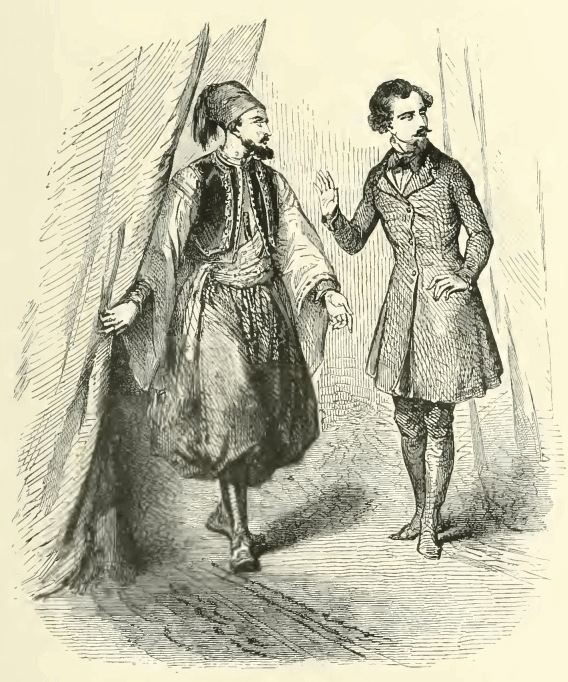
\includegraphics[width=\textwidth]{20079m.jpg}
\end{figure}

“Alas! I may say with Lucullus, if I could have anticipated the honor
of your visit, I would have prepared for it. But such as is my
hermitage, it is at your disposal; such as is my supper, it is yours to
share, if you will. Ali, is the supper ready?”

At this moment the tapestry moved aside, and a Nubian, black as ebony,
and dressed in a plain white tunic, made a sign to his master that all
was prepared in the dining-room.

“Now,” said the unknown to Franz, “I do not know if you are of my
opinion, but I think nothing is more annoying than to remain two or
three hours together without knowing by name or appellation how to
address one another. Pray observe, that I too much respect the laws of
hospitality to ask your name or title. I only request you to give me
one by which I may have the pleasure of addressing you. As for myself,
that I may put you at your ease, I tell you that I am generally called
‘Sinbad the Sailor.’”

“And I,” replied Franz, “will tell you, as I only require his wonderful
lamp to make me precisely like Aladdin, that I see no reason why at
this moment I should not be called Aladdin. That will keep us from
going away from the East whither I am tempted to think I have been
conveyed by some good genius.”

“Well, then, Signor Aladdin,” replied the singular Amphitryon, “you
heard our repast announced, will you now take the trouble to enter the
dining-room, your humble servant going first to show the way?”

At these words, moving aside the tapestry, Sinbad preceded his guest.
Franz now looked upon another scene of enchantment; the table was
splendidly covered, and once convinced of this important point he cast
his eyes around him. The dining-room was scarcely less striking than
the room he had just left; it was entirely of marble, with antique
bas-reliefs of priceless value; and at the four corners of this
apartment, which was oblong, were four magnificent statues, having
baskets in their hands. These baskets contained four pyramids of most
splendid fruit; there were Sicily pine-apples, pomegranates from
Malaga, oranges from the Balearic Isles, peaches from France, and dates
from Tunis.

The supper consisted of a roast pheasant garnished with Corsican
blackbirds; a boar’s ham with jelly, a quarter of a kid with tartar
sauce, a glorious turbot, and a gigantic lobster. Between these large
dishes were smaller ones containing various dainties. The dishes were
of silver, and the plates of Japanese china.

Franz rubbed his eyes in order to assure himself that this was not a
dream. Ali alone was present to wait at table, and acquitted himself so
admirably, that the guest complimented his host thereupon.

“Yes,” replied he, while he did the honors of the supper with much ease
and grace—“yes, he is a poor devil who is much devoted to me, and does
all he can to prove it. He remembers that I saved his life, and as he
has a regard for his head, he feels some gratitude towards me for
having kept it on his shoulders.”

Ali approached his master, took his hand, and kissed it.

“Would it be impertinent, Signor Sinbad,” said Franz, “to ask you the
particulars of this kindness?”

\begin{figure}[ht]
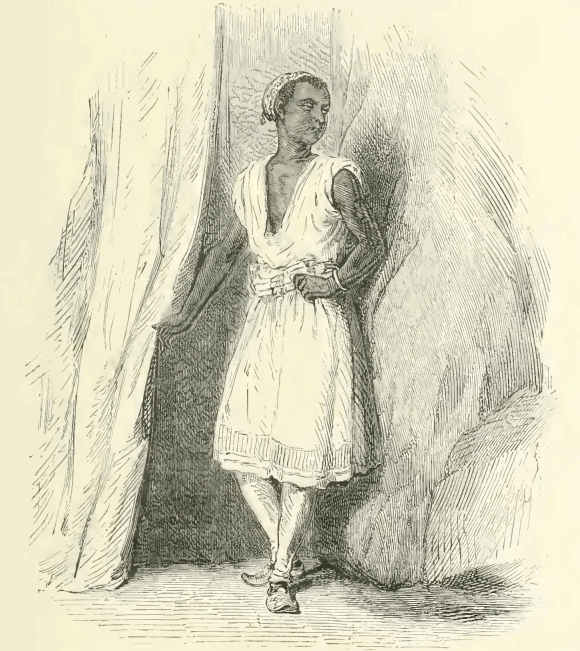
\includegraphics[width=\textwidth]{20081m.jpg}
\end{figure}

“Oh, they are simple enough,” replied the host. “It seems the fellow
had been caught wandering nearer to the harem of the Bey of Tunis than
etiquette permits to one of his color, and he was condemned by the Bey
to have his tongue cut out, and his hand and head cut off; the tongue
the first day, the hand the second, and the head the third. I always
had a desire to have a mute in my service, so learning the day his
tongue was cut out, I went to the Bey, and proposed to give him for Ali
a splendid double-barreled gun, which I knew he was very desirous of
having. He hesitated a moment, he was so very desirous to complete the
poor devil’s punishment. But when I added to the gun an English cutlass
with which I had shivered his highness’s yataghan to pieces, the Bey
yielded, and agreed to forgive the hand and head, but on condition that
the poor fellow never again set foot in Tunis. This was a useless
clause in the bargain, for whenever the coward sees the first glimpse
of the shores of Africa, he runs down below, and can only be induced to
appear again when we are out of sight of that quarter of the globe.”

Franz remained a moment silent and pensive, hardly knowing what to
think of the half-kindness, half-cruelty, with which his host related
the brief narrative.

“And like the celebrated sailor whose name you have assumed,” he said,
by way of changing the conversation, “you pass your life in
travelling?”

“Yes. I made a vow at a time when I little thought I should ever be
able to accomplish it,” said the unknown with a singular smile; “and I
made some others also which I hope I may fulfil in due season.”

Although Sinbad pronounced these words with much calmness, his eyes
gave forth gleams of extraordinary ferocity.

“You have suffered a great deal, sir?” said Franz inquiringly.

Sinbad started and looked fixedly at him, as he replied, “What makes
you suppose so?”

“Everything,” answered Franz,—“your voice, your look, your pallid
complexion, and even the life you lead.”

“I?—I live the happiest life possible, the real life of a pasha. I am
king of all creation. I am pleased with one place, and stay there; I
get tired of it, and leave it; I am free as a bird and have wings like
one; my attendants obey my slightest wish. Sometimes I amuse myself by
delivering some bandit or criminal from the bonds of the law. Then I
have my mode of dispensing justice, silent and sure, without respite or
appeal, which condemns or pardons, and which no one sees. Ah, if you
had tasted my life, you would not desire any other, and would never
return to the world unless you had some great project to accomplish
there.”

“Revenge, for instance!” observed Franz.

The unknown fixed on the young man one of those looks which penetrate
into the depth of the heart and thoughts. “And why revenge?” he asked.

“Because,” replied Franz, “you seem to me like a man who, persecuted by
society, has a fearful account to settle with it.”

“Ah!” responded Sinbad, laughing with his singular laugh, which
displayed his white and sharp teeth. “You have not guessed rightly.
Such as you see me I am, a sort of philosopher, and one day perhaps I
shall go to Paris to rival Monsieur Appert, and the man in the little
blue cloak.”

“And will that be the first time you ever took that journey?”

“Yes; it will. I must seem to you by no means curious, but I assure you
that it is not my fault I have delayed it so long—it will happen one
day or the other.”

\begin{figure}[ht]
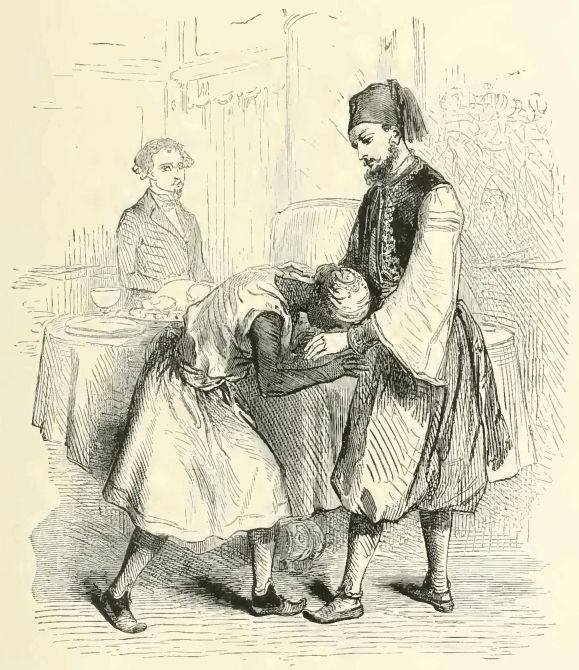
\includegraphics[width=\textwidth]{20083m.jpg}
\end{figure}

“And do you propose to make this journey very shortly?”

“I do not know; it depends on circumstances which depend on certain
arrangements.”

“I should like to be there at the time you come, and I will endeavor to
repay you, as far as lies in my power, for your liberal hospitality
displayed to me at Monte Cristo.”

“I should avail myself of your offer with pleasure,” replied the host,
“but, unfortunately, if I go there, it will be, in all probability,
\textit{incognito}.”

The supper appeared to have been supplied solely for Franz, for the
unknown scarcely touched one or two dishes of the splendid banquet to
which his guest did ample justice. Then Ali brought on the dessert, or
rather took the baskets from the hands of the statues and placed them
on the table. Between the two baskets he placed a small silver cup with
a silver cover. The care with which Ali placed this cup on the table
roused Franz’s curiosity. He raised the cover and saw a kind of
greenish paste, something like preserved angelica, but which was
perfectly unknown to him. He replaced the lid, as ignorant of what the
cup contained as he was before he had looked at it, and then casting
his eyes towards his host he saw him smile at his disappointment.

“You cannot guess,” said he, “what there is in that small vase, can
you?”

“No, I really cannot.”

“Well, then, that green preserve is nothing less than the ambrosia
which Hebe served at the table of Jupiter.”

“But,” replied Franz, “this ambrosia, no doubt, in passing through
mortal hands has lost its heavenly appellation and assumed a human
name; in vulgar phrase, what may you term this composition, for which,
to tell the truth, I do not feel any particular desire?”

“Ah, thus it is that our material origin is revealed,” cried Sinbad;
“we frequently pass so near to happiness without seeing, without
regarding it, or if we do see and regard it, yet without recognizing
it. Are you a man for the substantials, and is gold your god? taste
this, and the mines of Peru, Guzerat, and Golconda are opened to you.
Are you a man of imagination—a poet? taste this, and the boundaries of
possibility disappear; the fields of infinite space open to you, you
advance free in heart, free in mind, into the boundless realms of
unfettered reverie. Are you ambitious, and do you seek after the
greatnesses of the earth? taste this, and in an hour you will be a
king, not a king of a petty kingdom hidden in some corner of Europe
like France, Spain, or England, but king of the world, king of the
universe, king of creation; without bowing at the feet of Satan, you
will be king and master of all the kingdoms of the earth. Is it not
tempting what I offer you, and is it not an easy thing, since it is
only to do thus? look!”

At these words he uncovered the small cup which contained the substance
so lauded, took a teaspoonful of the magic sweetmeat, raised it to his
lips, and swallowed it slowly with his eyes half shut and his head bent
backwards. Franz did not disturb him whilst he absorbed his favorite
sweetmeat, but when he had finished, he inquired:

“What, then, is this precious stuff?”

“Did you ever hear,” he replied, “of the Old Man of the Mountain, who
attempted to assassinate Philippe Auguste?”

“Of course I have.”

“Well, you know he reigned over a rich valley which was overhung by the
mountain whence he derived his picturesque name. In this valley were
magnificent gardens planted by Hassen-ben-Sabah, and in these gardens
isolated pavilions. Into these pavilions he admitted the elect, and
there, says Marco Polo, gave them to eat a certain herb, which
transported them to Paradise, in the midst of ever-blooming shrubs,
ever-ripe fruit, and ever-lovely virgins. What these happy persons took
for reality was but a dream; but it was a dream so soft, so voluptuous,
so enthralling, that they sold themselves body and soul to him who gave
it to them, and obedient to his orders as to those of a deity, struck
down the designated victim, died in torture without a murmur, believing
that the death they underwent was but a quick transition to that life
of delights of which the holy herb, now before you, had given them a
slight foretaste.”

“Then,” cried Franz, “it is hashish! I know that—by name at least.”

“That is it precisely, Signor Aladdin; it is hashish—the purest and
most unadulterated hashish of Alexandria,—the hashish of Abou-Gor, the
celebrated maker, the only man, the man to whom there should be built a
palace, inscribed with these words, \textit{A grateful world to the dealer in
happiness}.”

“Do you know,” said Franz, “I have a very great inclination to judge
for myself of the truth or exaggeration of your eulogies.”

“Judge for yourself, Signor Aladdin—judge, but do not confine yourself
to one trial. Like everything else, we must habituate the senses to a
fresh impression, gentle or violent, sad or joyous. There is a struggle
in nature against this divine substance,—in nature which is not made
for joy and clings to pain. Nature subdued must yield in the combat,
the dream must succeed to reality, and then the dream reigns supreme,
then the dream becomes life, and life becomes the dream. But what
changes occur! It is only by comparing the pains of actual being with
the joys of the assumed existence, that you would desire to live no
longer, but to dream thus forever. When you return to this mundane
sphere from your visionary world, you would seem to leave a Neapolitan
spring for a Lapland winter—to quit paradise for earth—heaven for hell!
Taste the hashish, guest of mine—taste the hashish.”

Franz’s only reply was to take a teaspoonful of the marvellous
preparation, about as much in quantity as his host had eaten, and lift
it to his mouth.

“\textit{Diable!}” he said, after having swallowed the divine preserve. “I do
not know if the result will be as agreeable as you describe, but the
thing does not appear to me as palatable as you say.”

“Because your palate his not yet been attuned to the sublimity of the
substances it flavors. Tell me, the first time you tasted oysters, tea,
porter, truffles, and sundry other dainties which you now adore, did
you like them? Could you comprehend how the Romans stuffed their
pheasants with assafœtida, and the Chinese eat swallows’ nests? Eh? no!
Well, it is the same with hashish; only eat for a week, and nothing in
the world will seem to you to equal the delicacy of its flavor, which
now appears to you flat and distasteful. Let us now go into the
adjoining chamber, which is your apartment, and Ali will bring us
coffee and pipes.”

They both arose, and while he who called himself Sinbad—and whom we
have occasionally named so, that we might, like his guest, have some
title by which to distinguish him—gave some orders to the servant,
Franz entered still another apartment.

It was simply yet richly furnished. It was round, and a large divan
completely encircled it. Divan, walls, ceiling, floor, were all covered
with magnificent skins as soft and downy as the richest carpets; there
were heavy-maned lion-skins from Atlas, striped tiger-skins from
Bengal; panther-skins from the Cape, spotted beautifully, like those
that appeared to Dante; bear-skins from Siberia, fox-skins from Norway,
and so on; and all these skins were strewn in profusion one on the
other, so that it seemed like walking over the most mossy turf, or
reclining on the most luxurious bed.

Both laid themselves down on the divan; chibouques with jasmine tubes
and amber mouthpieces were within reach, and all prepared so that there
was no need to smoke the same pipe twice. Each of them took one, which
Ali lighted and then retired to prepare the coffee.

There was a moment’s silence, during which Sinbad gave himself up to
thoughts that seemed to occupy him incessantly, even in the midst of
his conversation; and Franz abandoned himself to that mute reverie,
into which we always sink when smoking excellent tobacco, which seems
to remove with its fume all the troubles of the mind, and to give the
smoker in exchange all the visions of the soul. Ali brought in the
coffee.

“How do you take it?” inquired the unknown; “in the French or Turkish
style, strong or weak, sugar or none, cool or boiling? As you please;
it is ready in all ways.”

“I will take it in the Turkish style,” replied Franz.

“And you are right,” said his host; “it shows you have a tendency for
an Oriental life. Ah, those Orientals; they are the only men who know
how to live. As for me,” he added, with one of those singular smiles
which did not escape the young man, “when I have completed my affairs
in Paris, I shall go and die in the East; and should you wish to see me
again, you must seek me at Cairo, Bagdad, or Ispahan.”

“\textit{Ma foi},” said Franz, “it would be the easiest thing in the world;
for I feel eagle’s wings springing out at my shoulders, and with those
wings I could make a tour of the world in four-and-twenty hours.”

“Ah, yes, the hashish is beginning its work. Well, unfurl your wings,
and fly into superhuman regions; fear nothing, there is a watch over
you; and if your wings, like those of Icarus, melt before the sun, we
are here to ease your fall.”

He then said something in Arabic to Ali, who made a sign of obedience
and withdrew, but not to any distance.

As to Franz a strange transformation had taken place in him. All the
bodily fatigue of the day, all the preoccupation of mind which the
events of the evening had brought on, disappeared as they do at the
first approach of sleep, when we are still sufficiently conscious to be
aware of the coming of slumber. His body seemed to acquire an airy
lightness, his perception brightened in a remarkable manner, his senses
seemed to redouble their power, the horizon continued to expand; but it
was not the gloomy horizon of vague alarms, and which he had seen
before he slept, but a blue, transparent, unbounded horizon, with all
the blue of the ocean, all the spangles of the sun, all the perfumes of
the summer breeze; then, in the midst of the songs of his
sailors,—songs so clear and sonorous, that they would have made a
divine harmony had their notes been taken down,—he saw the Island of
Monte Cristo, no longer as a threatening rock in the midst of the
waves, but as an oasis in the desert; then, as his boat drew nearer,
the songs became louder, for an enchanting and mysterious harmony rose
to heaven, as if some Loreley had decreed to attract a soul thither, or
Amphion, the enchanter, intended there to build a city.

At length the boat touched the shore, but without effort, without
shock, as lips touch lips; and he entered the grotto amidst continued
strains of most delicious melody. He descended, or rather seemed to
descend, several steps, inhaling the fresh and balmy air, like that
which may be supposed to reign around the grotto of Circe, formed from
such perfumes as set the mind a-dreaming, and such fires as burn the
very senses; and he saw again all he had seen before his sleep, from
Sinbad, his singular host, to Ali, the mute attendant; then all seemed
to fade away and become confused before his eyes, like the last shadows
of the magic lantern before it is extinguished, and he was again in the
chamber of statues, lighted only by one of those pale and antique lamps
which watch in the dead of the night over the sleep of pleasure.

They were the same statues, rich in form, in attraction, and poesy,
with eyes of fascination, smiles of love, and bright and flowing hair.
They were Phryne, Cleopatra, Messalina, those three celebrated
courtesans. Then among them glided like a pure ray, like a Christian
angel in the midst of Olympus, one of those chaste figures, those calm
shadows, those soft visions, which seemed to veil its virgin brow
before these marble wantons.

Then the three statues advanced towards him with looks of love, and
approached the couch on which he was reposing, their feet hidden in
their long white tunics, their throats bare, hair flowing like waves,
and assuming attitudes which the gods could not resist, but which
saints withstood, and looks inflexible and ardent like those with which
the serpent charms the bird; and then he gave way before looks that
held him in a torturing grasp and delighted his senses as with a
voluptuous kiss.

It seemed to Franz that he closed his eyes, and in a last look about
him saw the vision of modesty completely veiled; and then followed a
dream of passion like that promised by the Prophet to the elect. Lips
of stone turned to flame, breasts of ice became like heated lava, so
that to Franz, yielding for the first time to the sway of the drug,
love was a sorrow and voluptuousness a torture, as burning mouths were
pressed to his thirsty lips, and he was held in cool serpent-like
embraces. The more he strove against this unhallowed passion the more
his senses yielded to its thrall, and at length, weary of a struggle
that taxed his very soul, he gave way and sank back breathless and
exhausted beneath the kisses of these marble goddesses, and the
enchantment of his marvellous dream.
